% Options for packages loaded elsewhere
\PassOptionsToPackage{unicode}{hyperref}
\PassOptionsToPackage{hyphens}{url}
\PassOptionsToPackage{dvipsnames,svgnames,x11names}{xcolor}
%
\documentclass[
  singlecolumn]{report}

\usepackage{amsmath,amssymb}
\usepackage[]{libertinus}
\usepackage{iftex}
\ifPDFTeX
  \usepackage[T1]{fontenc}
  \usepackage[utf8]{inputenc}
  \usepackage{textcomp} % provide euro and other symbols
\else % if luatex or xetex
  \usepackage{unicode-math}
  \defaultfontfeatures{Scale=MatchLowercase}
  \defaultfontfeatures[\rmfamily]{Ligatures=TeX,Scale=1}
\fi
% Use upquote if available, for straight quotes in verbatim environments
\IfFileExists{upquote.sty}{\usepackage{upquote}}{}
\IfFileExists{microtype.sty}{% use microtype if available
  \usepackage[]{microtype}
  \UseMicrotypeSet[protrusion]{basicmath} % disable protrusion for tt fonts
}{}
\makeatletter
\@ifundefined{KOMAClassName}{% if non-KOMA class
  \IfFileExists{parskip.sty}{%
    \usepackage{parskip}
  }{% else
    \setlength{\parindent}{0pt}
    \setlength{\parskip}{6pt plus 2pt minus 1pt}}
}{% if KOMA class
  \KOMAoptions{parskip=half}}
\makeatother
\usepackage{xcolor}
\usepackage[top=30mm,left=20mm,heightrounded]{geometry}
\setlength{\emergencystretch}{3em} % prevent overfull lines
\setcounter{secnumdepth}{-\maxdimen} % remove section numbering
% Make \paragraph and \subparagraph free-standing
\ifx\paragraph\undefined\else
  \let\oldparagraph\paragraph
  \renewcommand{\paragraph}[1]{\oldparagraph{#1}\mbox{}}
\fi
\ifx\subparagraph\undefined\else
  \let\oldsubparagraph\subparagraph
  \renewcommand{\subparagraph}[1]{\oldsubparagraph{#1}\mbox{}}
\fi


\providecommand{\tightlist}{%
  \setlength{\itemsep}{0pt}\setlength{\parskip}{0pt}}\usepackage{longtable,booktabs,array}
\usepackage{calc} % for calculating minipage widths
% Correct order of tables after \paragraph or \subparagraph
\usepackage{etoolbox}
\makeatletter
\patchcmd\longtable{\par}{\if@noskipsec\mbox{}\fi\par}{}{}
\makeatother
% Allow footnotes in longtable head/foot
\IfFileExists{footnotehyper.sty}{\usepackage{footnotehyper}}{\usepackage{footnote}}
\makesavenoteenv{longtable}
\usepackage{graphicx}
\makeatletter
\def\maxwidth{\ifdim\Gin@nat@width>\linewidth\linewidth\else\Gin@nat@width\fi}
\def\maxheight{\ifdim\Gin@nat@height>\textheight\textheight\else\Gin@nat@height\fi}
\makeatother
% Scale images if necessary, so that they will not overflow the page
% margins by default, and it is still possible to overwrite the defaults
% using explicit options in \includegraphics[width, height, ...]{}
\setkeys{Gin}{width=\maxwidth,height=\maxheight,keepaspectratio}
% Set default figure placement to htbp
\makeatletter
\def\fps@figure{htbp}
\makeatother
\newlength{\cslhangindent}
\setlength{\cslhangindent}{1.5em}
\newlength{\csllabelwidth}
\setlength{\csllabelwidth}{3em}
\newlength{\cslentryspacingunit} % times entry-spacing
\setlength{\cslentryspacingunit}{\parskip}
\newenvironment{CSLReferences}[2] % #1 hanging-ident, #2 entry spacing
 {% don't indent paragraphs
  \setlength{\parindent}{0pt}
  % turn on hanging indent if param 1 is 1
  \ifodd #1
  \let\oldpar\par
  \def\par{\hangindent=\cslhangindent\oldpar}
  \fi
  % set entry spacing
  \setlength{\parskip}{#2\cslentryspacingunit}
 }%
 {}
\usepackage{calc}
\newcommand{\CSLBlock}[1]{#1\hfill\break}
\newcommand{\CSLLeftMargin}[1]{\parbox[t]{\csllabelwidth}{#1}}
\newcommand{\CSLRightInline}[1]{\parbox[t]{\linewidth - \csllabelwidth}{#1}\break}
\newcommand{\CSLIndent}[1]{\hspace{\cslhangindent}#1}

\usepackage{booktabs}
\usepackage{longtable}
\usepackage{array}
\usepackage{multirow}
\usepackage{wrapfig}
\usepackage{float}
\usepackage{colortbl}
\usepackage{pdflscape}
\usepackage{tabu}
\usepackage{threeparttable}
\usepackage{threeparttablex}
\usepackage[normalem]{ulem}
\usepackage{makecell}
\usepackage{xcolor}
\makeatletter
\makeatother
\makeatletter
\makeatother
\makeatletter
\@ifpackageloaded{caption}{}{\usepackage{caption}}
\AtBeginDocument{%
\ifdefined\contentsname
  \renewcommand*\contentsname{Table of contents}
\else
  \newcommand\contentsname{Table of contents}
\fi
\ifdefined\listfigurename
  \renewcommand*\listfigurename{List of Figures}
\else
  \newcommand\listfigurename{List of Figures}
\fi
\ifdefined\listtablename
  \renewcommand*\listtablename{List of Tables}
\else
  \newcommand\listtablename{List of Tables}
\fi
\ifdefined\figurename
  \renewcommand*\figurename{Figure}
\else
  \newcommand\figurename{Figure}
\fi
\ifdefined\tablename
  \renewcommand*\tablename{Table}
\else
  \newcommand\tablename{Table}
\fi
}
\@ifpackageloaded{float}{}{\usepackage{float}}
\floatstyle{ruled}
\@ifundefined{c@chapter}{\newfloat{codelisting}{h}{lop}}{\newfloat{codelisting}{h}{lop}[chapter]}
\floatname{codelisting}{Listing}
\newcommand*\listoflistings{\listof{codelisting}{List of Listings}}
\makeatother
\makeatletter
\@ifpackageloaded{caption}{}{\usepackage{caption}}
\@ifpackageloaded{subcaption}{}{\usepackage{subcaption}}
\makeatother
\makeatletter
\@ifpackageloaded{tcolorbox}{}{\usepackage[many]{tcolorbox}}
\makeatother
\makeatletter
\@ifundefined{shadecolor}{\definecolor{shadecolor}{rgb}{.97, .97, .97}}
\makeatother
\makeatletter
\makeatother
\ifLuaTeX
  \usepackage{selnolig}  % disable illegal ligatures
\fi
\IfFileExists{bookmark.sty}{\usepackage{bookmark}}{\usepackage{hyperref}}
\IfFileExists{xurl.sty}{\usepackage{xurl}}{} % add URL line breaks if available
\urlstyle{same} % disable monospaced font for URLs
\hypersetup{
  pdftitle={Who are the NFDS},
  pdfauthor={Authors TBA; Chris G Sibley; Joseph Bulbulia},
  pdfkeywords={Religious Change, Christianity, Denominations},
  colorlinks=true,
  linkcolor={blue},
  filecolor={Maroon},
  citecolor={Blue},
  urlcolor={Blue},
  pdfcreator={LaTeX via pandoc}}

\title{Who are the NFDS}
\usepackage{etoolbox}
\makeatletter
\providecommand{\subtitle}[1]{% add subtitle to \maketitle
  \apptocmd{\@title}{\par {\large #1 \par}}{}{}
}
\makeatother
\subtitle{An OutcomeWide Study}
\author{Authors TBA \and Chris G Sibley \and Joseph Bulbulia}
\date{3/29/23}

\begin{document}
\maketitle
\begin{abstract}
Who are the NFDs anyway?
\end{abstract}
\ifdefined\Shaded\renewenvironment{Shaded}{\begin{tcolorbox}[boxrule=0pt, interior hidden, enhanced, borderline west={3pt}{0pt}{shadecolor}, sharp corners, breakable, frame hidden]}{\end{tcolorbox}}\fi

\listoffigures
\listoftables
\hypertarget{introduction}{%
\section{Introduction}\label{introduction}}

Who are the NFDs anyway?(\protect\hyperlink{ref-sibley2012}{Sibley
2012})

\hypertarget{method}{%
\section{Method}\label{method}}

\hypertarget{questions-related-to-religion-are-as-follows}{%
\subsection{Questions related to religion are as
follows}\label{questions-related-to-religion-are-as-follows}}

\hypertarget{belief-in-god}{%
\subsubsection{Belief in God}\label{belief-in-god}}

Using one item from Eurobarometer (2005), we asked participants ``Do you
believe in a God'' (1 = Yes, 0 = No)
(\protect\hyperlink{ref-eurobarometer2005b}{Eurobarometer 2005}).

\hypertarget{belief-in-sprituality}{%
\subsubsection{Belief in Sprituality}\label{belief-in-sprituality}}

Using one item from Eurobarometer (2005), we asked participants ``Do you
believe in some form of spirit or lifeforce? (1 = Yes, 0 = No)
(\protect\hyperlink{ref-eurobarometer2005b}{Eurobarometer 2005}).

\hypertarget{religion-affiliation}{%
\subsubsection{Religion Affiliation}\label{religion-affiliation}}

Participants were asked to indicate their religion identification (``Do
you identify with a religion and/or spiritual group?'') on a binary
response (1 = Yes, 0 = No). We then asked ``What religion or spiritual
group?'' These questions are used in the New Zealand Census.

\hypertarget{frequency-of-church-attendence}{%
\subsubsection{Frequency of Church
Attendence}\label{frequency-of-church-attendence}}

If participants answered \emph{yes} to ``Do you identify with a religion
and/or spiritual group?'' we measured their frequency of church
attendance using one item from Sibley
(\protect\hyperlink{ref-sibley2012}{2012}): ``how many times did you
attend a church or place of worship in the last month?''. Those
participants who were not religious were imputed a score of ``0''.

\hypertarget{frequency-of-prayer}{%
\subsubsection{Frequency of Prayer}\label{frequency-of-prayer}}

If participants answered \emph{yes} to ``Do you identify with a religion
and/or spiritual group?'' we measured their frequency of prayer by
asking ``how many times did you pray in the last week?'' Those
participants who were not religious were imputed a score of ``0''
(\protect\hyperlink{ref-Bulbulia_2015}{S. Bulbulia J. A. 2015}) .

\hypertarget{frequency-of-scripture-reading}{%
\subsubsection{Frequency of Scripture
Reading}\label{frequency-of-scripture-reading}}

If participants answered \emph{yes} to ``Do you identify with a religion
and/or spiritual group?'' we measured their frequency of scripture
reading by asking ``how many times did you read religious scripture in
the last week?'' Those participants who were not religious were imputed
a score of ``0'' (\protect\hyperlink{ref-bulbulia2016}{J. Bulbulia et
al. 2016}).

\hypertarget{religious-identification}{%
\subsection{Religious Identification}\label{religious-identification}}

If participants answered \emph{yes} to ``Do you identify with a religion
and/or spiritual group? we asked''How important is your religion to how
you see yourself?'' (1 = Not important, 7 = Very important). Those
participants who were not religious were imputed a score of ``0''.

\hypertarget{descriptive-statistics}{%
\section{Descriptive statistics}\label{descriptive-statistics}}

\hypertarget{analytic-approach}{%
\subsection{Analytic approach}\label{analytic-approach}}

We next leveraged longitudinal data to investigate whether changing from
transiting from a Christian denomination to a Christian NFD affiliation
affect people's religious behaviors. That is, we used the longitudinal
features of NZAVS data collection to evalutate the causal question of
whether becoming a Christian NFD makes somebody less
religious.(\protect\hyperlink{ref-eurobarometer2005b}{Eurobarometer
2005})

\hypertarget{selection-criteria.}{%
\subsection{Selection criteria.}\label{selection-criteria.}}

\begin{enumerate}
\def\labelenumi{\arabic{enumi}.}
\tightlist
\item
  We selected people who participated in both the NZAVS 2018 and 2019
  waves.
\item
  We modelled religious behaviour as
\item
  Because non-response and panel attrition may bias estimates, we
  multiply impute missing data both in the Time 10 baseline and Time 11
  post-attack waves.
\item
  Using a repeated measures design, we naively assess the effects of the
  attack exposure on 2019/2020 (NZAVS Time 11) responses to all minority
  groups measure by the NZAVS estimating the effect of time on
  group-level attitudes. The NZAVS Time 10 pre-attack responses identify
  pre-exposure values; The NZAVS Time 11 post-attack responses identify
  post-attack attitudes. Note that in the naive analysis, the unit of
  time (one-year) is the exposure. Here we stimate the effect of time
  within individuals adjusting for the dependencies from the repeated
  measures using Generalised Estimating Equations (GEE)
  (\protect\hyperlink{ref-halekoh2006}{\textbf{halekoh2006?}}). To
  recover population-level coefficients we use sampling weights.
  (SUPPLEMENT XYZ describes estimates for the ATE, which are
  substantially similar.)
\item
  Recover the \textbf{Population Average Treatment Effect (PATE)} of the
  Attacks on Group Attitudes using G-computation:(a) compute the
  expected effect of the attack condition (exposure = 1) for the entire
  sample weighted by post-stratification sample weights. (b) compute the
  expected effect of the no-attack condition (exposure = 0) for the
  sample weighted by post-stratification sample weights. The difference
  in these expected values is the statistical estimate of the
  \textbf{PATE}. We obtain standard errors using the delta method and
  simulation-based inference
  (\protect\hyperlink{ref-greifer2023}{\textbf{greifer2023?}}).\footnote{We
    note that this coefficient is simply the time effect in the
    conditional analysis. We use G-computation for consistency with
    other NZAVS outcome-wide studies}.
\item
  Next, using this same sample, we obtain responses from prior to the
  attacks: years 2016-2019 (pre-attack). Again we multiply-impute
  missing values for missing responses conditional on demographic,
  political, and personality indicators.
\item
  We estimate the time trend from these years for each of the 12 social
  attitude domains.
\item
  We use the average, lower, upper intervals of these estimates to
  obtain bounds with which to adjust the estimated effects of the
  attacks of social attitudes from the naive analysis. These adjustments
  represent the best, worst-case scenarios for the attack-effect
  estimands. Again because it is preferable to think of social attitudes
  as increasing without a focus on injustice, we describe the outcomes
  adjusted under the strongest pre-attack intervals as ``best-case''
  outcomes for the attack effects, even if these attenuate the attack
  effect estimands.
\end{enumerate}

\hypertarget{sample}{%
\subsection{Sample}\label{sample}}

\hypertarget{tbl-sample}{}
\begin{longtable}[]{@{}ll@{}}
\caption{\label{tbl-sample}Sample Statistics (baseline =
2018)}\tabularnewline
\toprule()
& Time 10 (baseline) \\
\midrule()
\endfirsthead
\toprule()
& Time 10 (baseline) \\
\midrule()
\endhead
& (N=10787) \\
\textbf{Male} & \\
Male & 4003 (37 \%) \\
Not\_male & 6784 (63 \%) \\
\textbf{Cohort} & \\
Gen\_Silent: born\textless{} 1946 & 714 (7 \%) \\
Gen Boomers: born \textgreater= 1946 \& b.\textless{} 1965 & 5229 (48
\%) \\
GenX: born \textgreater=1961 \& b.\textless{} 1981 & 3311 (31 \%) \\
GenY: born \textgreater=1981 \& b.\textless{} 1996 & 1421 (13 \%) \\
GenZ: born \textgreater= 1996 & 112 (1 \%) \\
\textbf{NZ-European} & \\
No & 2018 (19 \%) \\
Yes & 8730 (81 \%) \\
Missing & 39 (0.4\%) \\
\textbf{Education} & \\
Mean (SD) & 5.63 (± 2.66) \\
Missing & 37 (0.3\%) \\
\textbf{Employed} & \\
No & 2714 (25 \%) \\
Yes & 8064 (75 \%) \\
Missing & 9 (0.1\%) \\
\textbf{NZDep2018} & \\
Mean (SD) & 4.70 (± 2.73) \\
Missing & 117 (1.1\%) \\
\textbf{NZSEI13} & \\
Mean (SD) & 54.9 (± 16.0) \\
Missing & 56 (0.5\%) \\
\textbf{Rural\_GCH2018} & \\
1 & 6632 (61 \%) \\
2 & 2092 (19 \%) \\
3 & 1254 (12 \%) \\
4 & 567 (5 \%) \\
5 & 126 (1 \%) \\
Missing & 116 (1.1\%) \\
\textbf{Born NZ} & \\
Mean (SD) & 0.800 (± 0.400) \\
Missing & 18 (0.2\%) \\
\textbf{Parent} & \\
No & 2574 (24 \%) \\
Yes & 8212 (76 \%) \\
Missing & 1 (0.0\%) \\
\textbf{Partner} & \\
No & 2576 (24 \%) \\
Yes & 7903 (73 \%) \\
Missing & 308 (2.9\%) \\
\textbf{Politically\_Liberal} & \\
Mean (SD) & 3.57 (± 1.38) \\
Missing & 497 (4.6\%) \\
\textbf{Left\_Wing} & \\
Mean (SD) & 3.71 (± 1.31) \\
Missing & 537 (5.0\%) \\
\textbf{Religious\_Identification} & \\
Mean (SD) & 1.72 (± 2.58) \\
Missing & 68 (0.6\%) \\
\bottomrule()
\end{longtable}

\hypertarget{description-of-changes-in-attitudes-in-sample-pre-post-attacks-one-year}{%
\subsection{Description of Changes in Attitudes in Sample Pre-Post
Attacks (one
year)}\label{description-of-changes-in-attitudes-in-sample-pre-post-attacks-one-year}}

The sample consists of 10,878 participants who responded the NZAVS
2016/17 Time 8 survey and who again responded to the NZAVS 2018/19 Time
10 survey.

\hypertarget{tbl-warmth}{}
\begin{longtable}[]{@{}
  >{\raggedright\arraybackslash}p{(\columnwidth - 4\tabcolsep) * \real{0.3571}}
  >{\raggedright\arraybackslash}p{(\columnwidth - 4\tabcolsep) * \real{0.3143}}
  >{\raggedright\arraybackslash}p{(\columnwidth - 4\tabcolsep) * \real{0.3286}}@{}}
\caption{\label{tbl-warmth}Average warmth ratings before and one-year
after attacks}\tabularnewline
\toprule()
\begin{minipage}[b]{\linewidth}\raggedright
\end{minipage} & \begin{minipage}[b]{\linewidth}\raggedright
Pre Attacks(Time 10)
\end{minipage} & \begin{minipage}[b]{\linewidth}\raggedright
Post Attacks(Time 11)
\end{minipage} \\
\midrule()
\endfirsthead
\toprule()
\begin{minipage}[b]{\linewidth}\raggedright
\end{minipage} & \begin{minipage}[b]{\linewidth}\raggedright
Pre Attacks(Time 10)
\end{minipage} & \begin{minipage}[b]{\linewidth}\raggedright
Post Attacks(Time 11)
\end{minipage} \\
\midrule()
\endhead
& (N=10787) & (N=10787) \\
\textbf{Warm Muslims} & & \\
Mean (SD) & 4.09 (1.46) & 4.35 (1.41) \\
Median {[}Min, Max{]} & 4.00 {[}1.00, 7.00{]} & 4.00 {[}1.00, 7.00{]} \\
Missing & 286 (2.7\%) & 1672 (15.5\%) \\
\textbf{Warm Asians} & & \\
Mean (SD) & 4.54 (1.27) & 4.64 (1.23) \\
Median {[}Min, Max{]} & 4.00 {[}1.00, 7.00{]} & 4.00 {[}1.00, 7.00{]} \\
Missing & 265 (2.5\%) & 1647 (15.3\%) \\
\textbf{Warm Chinese} & & \\
Mean (SD) & 4.39 (1.34) & 4.47 (1.32) \\
Median {[}Min, Max{]} & 4.00 {[}1.00, 7.00{]} & 4.00 {[}1.00, 7.00{]} \\
Missing & 280 (2.6\%) & 1673 (15.5\%) \\
\textbf{Warm Immigrants} & & \\
Mean (SD) & 4.54 (1.23) & 4.64 (1.23) \\
Median {[}Min, Max{]} & 4.00 {[}1.00, 7.00{]} & 4.00 {[}1.00, 7.00{]} \\
Missing & 282 (2.6\%) & 1674 (15.5\%) \\
\textbf{Warm Indians} & & \\
Mean (SD) & 4.31 (1.36) & 4.42 (1.34) \\
Median {[}Min, Max{]} & 4.00 {[}1.00, 7.00{]} & 4.00 {[}1.00, 7.00{]} \\
Missing & 277 (2.6\%) & 1669 (15.5\%) \\
\textbf{Warm Refugees} & & \\
Mean (SD) & 4.68 (1.34) & 4.80 (1.31) \\
Median {[}Min, Max{]} & 5.00 {[}1.00, 7.00{]} & 5.00 {[}1.00, 7.00{]} \\
Missing & 283 (2.6\%) & 1654 (15.3\%) \\
\textbf{Warm Pacific} & & \\
Mean (SD) & 4.78 (1.24) & 4.87 (1.20) \\
Median {[}Min, Max{]} & 5.00 {[}1.00, 7.00{]} & 5.00 {[}1.00, 7.00{]} \\
Missing & 265 (2.5\%) & 1654 (15.3\%) \\
\textbf{Warm Maori} & & \\
Mean (SD) & 5.00 (1.27) & 5.03 (1.26) \\
Median {[}Min, Max{]} & 5.00 {[}1.00, 7.00{]} & 5.00 {[}1.00, 7.00{]} \\
Missing & 270 (2.5\%) & 1660 (15.4\%) \\
\textbf{Warm NZ Euro} & & \\
Mean (SD) & 5.57 (1.23) & 5.58 (1.24) \\
Median {[}Min, Max{]} & 6.00 {[}1.00, 7.00{]} & 6.00 {[}1.00, 7.00{]} \\
Missing & 282 (2.6\%) & 1659 (15.4\%) \\
\textbf{Warm Elderly} & & \\
Mean (SD) & 5.52 (1.16) & 5.51 (1.15) \\
Median {[}Min, Max{]} & 6.00 {[}1.00, 7.00{]} & 6.00 {[}1.00, 7.00{]} \\
Missing & 258 (2.4\%) & 1648 (15.3\%) \\
\textbf{Warm Overweight} & & \\
Mean (SD) & 4.21 (1.37) & 4.22 (1.38) \\
Median {[}Min, Max{]} & 4.00 {[}1.00, 7.00{]} & 4.00 {[}1.00, 7.00{]} \\
Missing & 274 (2.5\%) & 1660 (15.4\%) \\
\textbf{Warm Mental-illness} & & \\
Mean (SD) & 4.60 (1.29) & 4.64 (1.28) \\
Median {[}Min, Max{]} & 4.00 {[}1.00, 7.00{]} & 4.00 {[}1.00, 7.00{]} \\
Missing & 288 (2.7\%) & 1671 (15.5\%) \\
\bottomrule()
\end{longtable}

\hypertarget{tbl-personality}{}
\begin{longtable}[]{@{}ll@{}}
\caption{\label{tbl-personality}Personality ratings at baseline. In
addition to demographic indicators we also used personality ratings to
multiply impute missing values}\tabularnewline
\toprule()
& Time 10 (baseline) \\
\midrule()
\endfirsthead
\toprule()
& Time 10 (baseline) \\
\midrule()
\endhead
& (N=10787) \\
AGREEABLENESS & \\
Mean (SD) & 5.36 (± 0.968) \\
Missing & 36 (0.3\%) \\
CONSCIENTIOUSNESS & \\
Mean (SD) & 5.15 (± 1.01) \\
Missing & 33 (0.3\%) \\
EXTRAVERSION & \\
Mean (SD) & 3.85 (± 1.16) \\
Missing & 33 (0.3\%) \\
HONESTY\_HUMILITY & \\
Mean (SD) & 5.51 (± 1.16) \\
Missing & 33 (0.3\%) \\
NEUROTICISM & \\
Mean (SD) & 3.38 (± 1.15) \\
Missing & 36 (0.3\%) \\
OPENNESS & \\
Mean (SD) & 4.95 (± 1.12) \\
Missing & 33 (0.3\%) \\
\bottomrule()
\end{longtable}

\hypertarget{selection-bias}{%
\subsection{Selection Bias}\label{selection-bias}}

Although the timing of the attacks was random with respect to NAVS data
collection, non-response and panel attrition may potentially bias
inferences. A simple version of this threat is indicated in
Figure~\ref{fig-dag}. \(\dots\). We used both demographic indicators
(see Table~\ref{tbl-sample}) and personality indicators (see
Table~\ref{tbl-personality}) when multiply imputing missing responses.

\begin{figure}

{\centering 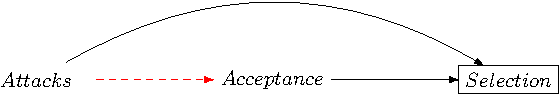
\includegraphics[width=0.8\textwidth,height=\textheight]{gt-manuscript_files/figure-pdf/fig-dag-1.pdf}

}

\caption{\label{fig-dag}Causal graph shows potential for selection bias
from loss to follow up or non-response. To address this, we multiply
impute missing values conditional on the assumption that missing values
are random conditional on the imputation model (MAR).}

\end{figure}

\hypertarget{results}{%
\section{Results}\label{results}}

Causal effect estimates on the difference scale are presented in
Figure~\ref{fig-results1}. Contrasts are presented in standardised
response units. Again, these causal effect estimates are modelled as a
contrast in (1) expected group attitudes for the entire population prior
to the attacks (NZAVS Time 10 pre-attacks) with (2) expected group
attitudes for the entire population during the following year weighted
by 2018 census data to recover post-stratification estimates. Assuming
correct model specification and no measurement error, such contrasts
would be unbiased estimates for the intention-to-treat effect for random
``assignment'' to the attack condition. {[}Note: see supplement X for a
discussion of the distinction between the per-protocol and intention to
treat effects{]}. Note that standard errors were obtained both by
simulation and the delta method (simulated contrasts are reported here.)
As indicated in Figure~\ref{fig-results1}, we replicate previous
findings revealing a strong increase in the acceptance of Muslims.
Furthermore, we find evidence for the transference of acceptance to
prototypical minorities. We do not find a boost in acceptance for
non-prototypical minority groups. Nor do we find acceptance for groups
that may be regarded as ``negative controls.'' The exception to this
pattern is in evidence of an increase in the acceptance of Pacific
peoples. Additionally, we find evidence for acceptance of those with
mentally illness.

Before attempting to interpret the naive analysis, however, we must
adjust for the possibility of temporal trends (see:
Table~\ref{tbl-timeproto}, Table~\ref{tbl-timenegcontrol},
Table~\ref{tbl-timenonproto}.)

\begin{figure}

{\centering \includegraphics{fig_1.jpg}

}

\caption{\label{fig-results1}Causal effect estimates on the difference
scale. Estimates were modelled with post-stratification survey weights
(Age/Gender/NZ European Ethnicity), yeilding a population average
treatment effect. However, these naive contrasts do not incorporate
pre-attack time trends in minority-group acceptance.}

\end{figure}

\begin{figure}

{\centering \includegraphics{fig_2.jpg}

}

\caption{\label{fig-results2}Sensitivity analysis for causal contrasts
adjusted for the estimated time trends in minority-group acceptance.
Panel (a) presents the ``worst case'' scenario for increasing acceptance
in pre-attack trajectories, implying that the attacks would have
increased acceptance for all groups. Panel (b) presents the scenario in
which increasing acceptance in pre-attack trajectories adjusted at the
mean of the pre-attack trends. Here we find stronger evidence for
transference of acceptance to non-prototypical groups. Panel (c)
presents the ``best case'' scenario for increasing acceptance in
pre-attack acceptance, implying that the attacks did not increase
acceptance as strongly as would appear in the naive analysis}

\end{figure}

Figure~\ref{fig-results2} presents a sensitivity analysis for causal
effect estimates on the difference scale. Panel (a) presents the ``worst
case'' scenario for increasing acceptance in pre-attack trajectories,
implying that the attacks would have increased acceptance for all
groups. This finding would be consistent with a strong ``Jacidina
Effect'' (see Discussion.)

Panel (b) presents the scenario in which increasing acceptance in
pre-attack trajectories adjusted at the mean of the pre-attack trends.
Here we find stronger evidence for the transference of acceptance to
non-prototypical groups. Panel (c) presents the ``best case'' scenario
for increasing acceptance in pre-attack acceptance, implying that the
attacks did not increase acceptance as strongly as would appear in the
naive analysis. Prototypical Attitude Response Theory survives the
strongest estimate of the pre-attack increase in acceptance. For this
reason our most conservative estimats supports Prototypical Attitude
Response Theory. Notably, at every level of the sensitivity analysis,
the causal effects of attitudes to Muslims are estimated lower than in
the naive analysis. This is because the acceptance of Muslims had been
growing more steeply in the years prior to the attacks than had the
acceptance of other groups. Notably, we find that as people age, they
tend to be less accepting of the elderly and of the dominant NZ European
majority.

\hypertarget{tbl-timeproto}{}
\begin{longtable}[]{@{}
  >{\raggedright\arraybackslash}p{(\columnwidth - 12\tabcolsep) * \real{0.1429}}
  >{\raggedright\arraybackslash}p{(\columnwidth - 12\tabcolsep) * \real{0.1429}}
  >{\raggedright\arraybackslash}p{(\columnwidth - 12\tabcolsep) * \real{0.1429}}
  >{\raggedleft\arraybackslash}p{(\columnwidth - 12\tabcolsep) * \real{0.1429}}
  >{\raggedright\arraybackslash}p{(\columnwidth - 12\tabcolsep) * \real{0.1429}}
  >{\raggedleft\arraybackslash}p{(\columnwidth - 12\tabcolsep) * \real{0.1429}}
  >{\raggedright\arraybackslash}p{(\columnwidth - 12\tabcolsep) * \real{0.1429}}@{}}
\caption{\label{tbl-timeproto}Estimated annual increase in acceptance
for prototypical minority groups. Note that attitudes to refugees were
not measured in the 2016/17 NZAVS Wave, rendering estimates for this
trajectory less reliable than other estimates.}\tabularnewline
\toprule()
\begin{minipage}[b]{\linewidth}\raggedright
Parameter
\end{minipage} & \begin{minipage}[b]{\linewidth}\raggedright
Muslims
\end{minipage} & \begin{minipage}[b]{\linewidth}\raggedright
Indians
\end{minipage} & \begin{minipage}[b]{\linewidth}\raggedleft
Asians
\end{minipage} & \begin{minipage}[b]{\linewidth}\raggedright
Refugees
\end{minipage} & \begin{minipage}[b]{\linewidth}\raggedleft
Immigrants
\end{minipage} & \begin{minipage}[b]{\linewidth}\raggedright
Chinese
\end{minipage} \\
\midrule()
\endfirsthead
\toprule()
\begin{minipage}[b]{\linewidth}\raggedright
Parameter
\end{minipage} & \begin{minipage}[b]{\linewidth}\raggedright
Muslims
\end{minipage} & \begin{minipage}[b]{\linewidth}\raggedright
Indians
\end{minipage} & \begin{minipage}[b]{\linewidth}\raggedleft
Asians
\end{minipage} & \begin{minipage}[b]{\linewidth}\raggedright
Refugees
\end{minipage} & \begin{minipage}[b]{\linewidth}\raggedleft
Immigrants
\end{minipage} & \begin{minipage}[b]{\linewidth}\raggedright
Chinese
\end{minipage} \\
\midrule()
\endhead
time & 0.05 (0.04, 0.06) & 0.02 (7.24e-03, 0.03) & 4.55e-03 (-6.34e-03,
0.02) & 0.01 (2.16e-04, 0.03) & 6.38e-03 (-4.39e-03, 0.02) & 0.01
(3.66e-03, 0.02) \\
\bottomrule()
\end{longtable}

\hypertarget{tbl-timenonproto}{}
\begin{longtable}[]{@{}
  >{\raggedright\arraybackslash}p{(\columnwidth - 6\tabcolsep) * \real{0.2466}}
  >{\raggedleft\arraybackslash}p{(\columnwidth - 6\tabcolsep) * \real{0.2466}}
  >{\raggedleft\arraybackslash}p{(\columnwidth - 6\tabcolsep) * \real{0.2466}}
  >{\raggedleft\arraybackslash}p{(\columnwidth - 6\tabcolsep) * \real{0.2603}}@{}}
\caption{\label{tbl-timenonproto}Estimated annual increase in acceptance
for non-prototypical groups}\tabularnewline
\toprule()
\begin{minipage}[b]{\linewidth}\raggedright
Parameter
\end{minipage} & \begin{minipage}[b]{\linewidth}\raggedleft
Pacific
\end{minipage} & \begin{minipage}[b]{\linewidth}\raggedleft
NZ European
\end{minipage} & \begin{minipage}[b]{\linewidth}\raggedleft
Maori
\end{minipage} \\
\midrule()
\endfirsthead
\toprule()
\begin{minipage}[b]{\linewidth}\raggedright
Parameter
\end{minipage} & \begin{minipage}[b]{\linewidth}\raggedleft
Pacific
\end{minipage} & \begin{minipage}[b]{\linewidth}\raggedleft
NZ European
\end{minipage} & \begin{minipage}[b]{\linewidth}\raggedleft
Maori
\end{minipage} \\
\midrule()
\endhead
(Intercept) & 0.004 (-0.02, 0.02) & 0.035 (0.01, 0.06) & 0.011 (-0.01,
0.03) \\
time & -0.010 (-0.02, 6.86e-04) & -0.034 (-0.05, -0.02) & -0.016 (-0.03,
-4.92e-03) \\
\bottomrule()
\end{longtable}

\hypertarget{tbl-timenegcontrol}{}
\begin{longtable}[]{@{}
  >{\raggedright\arraybackslash}p{(\columnwidth - 6\tabcolsep) * \real{0.2466}}
  >{\raggedright\arraybackslash}p{(\columnwidth - 6\tabcolsep) * \real{0.2466}}
  >{\raggedright\arraybackslash}p{(\columnwidth - 6\tabcolsep) * \real{0.2466}}
  >{\raggedleft\arraybackslash}p{(\columnwidth - 6\tabcolsep) * \real{0.2603}}@{}}
\caption{\label{tbl-timenegcontrol}Estimated annual increase in
acceptance for negative controls. Note that attitudes to those with
Mental Illness were not measured in the 2016/17 NZAVS Wave, rendering
estimates for this trajectory less reliable than other
estimates}\tabularnewline
\toprule()
\begin{minipage}[b]{\linewidth}\raggedright
Parameter
\end{minipage} & \begin{minipage}[b]{\linewidth}\raggedright
Overweight
\end{minipage} & \begin{minipage}[b]{\linewidth}\raggedright
Mental Illness
\end{minipage} & \begin{minipage}[b]{\linewidth}\raggedleft
Elderly
\end{minipage} \\
\midrule()
\endfirsthead
\toprule()
\begin{minipage}[b]{\linewidth}\raggedright
Parameter
\end{minipage} & \begin{minipage}[b]{\linewidth}\raggedright
Overweight
\end{minipage} & \begin{minipage}[b]{\linewidth}\raggedright
Mental Illness
\end{minipage} & \begin{minipage}[b]{\linewidth}\raggedleft
Elderly
\end{minipage} \\
\midrule()
\endhead
time & -0.006 (-0.02, 4.98e-03) & 0.010 (-6.45e-03, 0.03) & -0.023
(-0.04, -7.72e-03) \\
\bottomrule()
\end{longtable}

\hypertarget{discussion}{%
\section{Discussion}\label{discussion}}

Points to consider:

\begin{itemize}
\tightlist
\item
  Muslim acceptance post attacks is evident whether the pre-attack
  acceptance trend is bounded at its highest or lowest confidence
  interval.
\item
  Prototypical minority acceptance is also evident whether the
  pre-attack acceptance trend is bounded at its highest or lowest
  confidence interval.
\item
  The magnitude of prototypical minority acceptance is about half that
  of the Muslim acceptance post-attack benefit.
\item
  At the lower bound of the pre-attack acceptance trajectory, all groups
  experience a lift in post-attack acceptance. This scenario suggests
  the potential for a ``Jacinda Effect''.
\item
  However, the complex interplay of social events at that time in New
  Zealand History remains unclear -- and cannot be disentangled from
  observed data.\(\dots\)
\item
  At the upper bound of the pre-attack acceptance trajectory, only
  prototypical minority groups saw a lift in acceptance over and above
  expectations from the pre-attack trajectory.
\item
  Notably, although the confidence intervals for prototypical minorities
  were reliably above zero on this ``best-case'' pre-attack trajectory,
  the confidence intervals between prototypical and non-prototypical
  minority groups overlapped. We can therefore infer only somewhat weak
  overall support for prototyping in the attack responses.
\item
  This study reveals the potential for psychological science to reframe
  how popolar understandings of minority groups. In New Zealand Pacific
  peoples tend to be grouped with Māori peoples. However, the pattern of
  response to Pacific peoples following the Christchurch attacks is more
  closely aligned with the prototypical minority group response.
\item
  Moreover, the declining acceptance of elderly people and for New
  Zealand Europeans over time merits further attention. Overall
  acceptance of these populations remains the highest of all groups. The
  pattern does not necessarily imply increasing prejudice: it may rather
  reflect declining affective responses to the familar. Whether and how
  people naturally become less ``warm'' to others as we age is another
  matter for future investigations.
\item
  Overall this study reveals both the power and the limitations of
  longitudinal data to address questions of fundamental interest across
  the social sciences.
\item
\end{itemize}

\hypertarget{acknowledgments}{%
\section{Acknowledgments}\label{acknowledgments}}

HERE\ldots{}

\hypertarget{references}{%
\section{References}\label{references}}

\hypertarget{refs}{}
\begin{CSLReferences}{1}{0}
\leavevmode\vadjust pre{\hypertarget{ref-bulbulia2016}{}}%
Bulbulia, Joseph, Geoffrey Troughton, Lara M. Greaves, Taciano L.
Milfont, and Chris G. Sibley. 2016. {``To Burn or to Save? The Opposing
Functions of Reading Scripture on Environmental Intentions.''}
\emph{Religion, Brain \& Behavior} 6 (4): 278--89.
\url{https://doi.org/10.1080/2153599X.2015.1026926}.

\leavevmode\vadjust pre{\hypertarget{ref-Bulbulia_2015}{}}%
Bulbulia, Shaver, J. A. 2015. {``Religion and Parental Cooperation: An
Empirical Test of Slone's Sexual Signaling Model.''} In \emph{The
Attraction of Religion: A Sexual Selectionist Account}, edited by \& Van
Slyke J. Slone D., 29--62. Bloomsbury Press.

\leavevmode\vadjust pre{\hypertarget{ref-eurobarometer2005b}{}}%
Eurobarometer, Special. 2005. {``Social Values, Science and
Technology.''} \emph{Eurobarometer Special Report} 225.

\leavevmode\vadjust pre{\hypertarget{ref-sibley2012}{}}%
Sibley, \& Bulbulia, C. G. 2012. {``Healing Those Who Need Healing: How
Religious Practice Affects Social Belonging.''} \emph{Journal for the
Cognitive Science of Religion} 1: 29--45.

\end{CSLReferences}



\end{document}
